\chapter{Ассимптотически оптимальные оценки.}

\section{Сходимости, лемма Слуцкого} %\label{lec:1/sec:1}

Пусть случайные величины $\xi_n, \xi \in \mathbb{R}^n$ определены на колмогоровой тройке $(\Omega, F, P)$.
$F_n (x)$ - функция распределения $\xi_n$, $\varphi_n (t)$ - характеристическая функция, $Q_n$ - распределение (мера на множестве борелевских подмножеств).

\begin{definition}\label{lec:1/def:1}
	Говорят, что $F_n$ сходится к $F$ \red{в основном} ($F_n(x) \Rightarrow F(x)$), если $F_n(x) \to F(x) \; \forall x \in \mathbb{C}(F)$.
\end{definition}

\begin{definition}\label{lec:1/def:2}
	Говорят, что $Q_n$ сходится \red{слабо} к $Q$ ($Q_n \xrightarrow[]{W} Q$), если для любой непрерывной и ограниченной функции $g: \mathbb{R}^k \to \mathbb{R}^1$
	$$\underset{\mathbb{R}^k}{\overset{}{\int}}g(x) Q_n(dx) \to \underset{\mathbb{R}^1}{\overset{}{\int}}g(x) Q(dx) \; \Leftrightarrow \; E g(\xi_n) \to E g(\xi)$$ 
\end{definition}

\begin{theorem}[]\label{lec:1/the:1}
	Следующие условия эквивалентны:
	\begin{enumerate}
		\item $F_n \Rightarrow F$
		\item $Q_n \xrightarrow[]{W} Q$
		\item $\varphi_n (t) \to \varphi (t) \; \forall t \in \mathbb{R}^k$
	\end{enumerate}
\end{theorem}

\begin{definition}\label{lec:1/def:3}
	Если выполнено одно из условий $1)-3)$ из предыдущей теоремы, то говорят, что $\xi_n$ сходится к $\xi$ \red{по распределению} ($\xi_n \xrightarrow[]{d}\xi$). 
\end{definition}

\begin{theorem}[\blue{о наследовании сходимости}]\label{lec:1/the:2}
	Пусть $\xi_n, \xi \in \mathbb{R}^k$ и отображение $H: \mathbb{R}^k \to \mathbb{R}^1$ непрерывно. Тогда:
	\begin{enumerate}
		\item если $\xi_n \xrightarrow[]{d} \xi$, то $H(\xi_n) \xrightarrow[]{d} H(\xi)$
		\item если $\xi_n \xrightarrow[]{P} \xi$, то $H(\xi_n) \xrightarrow[]{P} H(\xi)$
	\end{enumerate}
\end{theorem}

\newpage
\begin{lemma}[\blue{Слуцкого}]\label{lec:1/lemma:1}
	Пусть $\xi_n, \xi, \eta_n, a \in \mathbb{R}^1$ и $\xi_n \xrightarrow[]{d}\xi, \eta_n \xrightarrow[]{P} a$. Тогда:
	\begin{itemize}
		\item[$\RNumb{1})$] $\xi_n + \eta_n \xrightarrow[]{d} \xi + a$
		\item[$\RNumb{2})$] $\xi_n \eta_n \xrightarrow[]{d} a \xi$
	\end{itemize}
\end{lemma}
\begin{Proof}
	Достаточно, чтобы была следующая сходимость:
	$$(\xi_n, \eta_n)^T \xrightarrow[]{d} (\xi, a)^T\eqno(1)$$
	Действительно, если $(1)$ верно, то при $H(x,y) = x+y$ по теореме $1.2$ получаем $\RNumb{1}$, а при $H(x,y) = xy$ получаем $\RNumb{2}$.

	Докажем $(1): \; (\xi_n, \eta_n)^T \xrightarrow[]{d}(\xi, a)^T$. Проверим, что характеристическая функция $(\xi_n, \eta_n)^T$ сходится к характеристической функции $(\xi, a)^T$:
	$$|E e^{i t \xi_n + i s \eta_n} - E e^{i t \xi + i s a}| \le |E e^{i t \xi_n + i s \eta_n} - E e^{i t \xi_n + i s a}| + |E e^{i t \xi_n + i s a} - E e^{i t \xi + i s a}| = \alpha_n + \beta_n$$
	$$\begin{gathered}
	\alpha_n \le E|e^{i t \xi_n} (e^{i s \eta_n} - e^{i s a})| = E|e^{i s \eta_n} - e^{i s a}| = E g(\eta_n) \\ 
	g(x) = |e^{i s x} - e^{i s a}| \text{ - непрерывная и ограниченная}, \; \eta_n \xrightarrow[]{d} a \; \Rightarrow \\
	\text{по теореме } 1.2 \;\; E g(\eta_n) \to E g(a) = 0 \; \Rightarrow \; \alpha_n \to 0
	\end{gathered}$$
	$$\begin{gathered}
		\beta_n = |E e^{i s a} (e^{i t \xi_n} - e^{i t \xi})| = |e^{i s a} E (e^{i t \xi_n} - e^{i t \xi})| = |E e^{i t \xi_n} - E e^{i t \xi}| \to 0, \text{ т.к. } \xi_n \xrightarrow[]{d}\xi.
	\end{gathered}$$

	Т.о. $\varphi_n (t) \to \varphi (t)$.
\end{Proof}

\section{Асимптотически нормальные, состоятельные оценки, асимптотический доверительный интервал}\label{lec:1/sec:2}

Пусть наблюдение $X \sim P_{\theta}, \; \theta \in \Theta \subseteq \mathbb{R}^k$. $\hat{\theta_n}$ - оценка $\theta$.

\begin{definition}\label{lec:1/def:4}
	Если $\sqrt{n} (\hat{\theta_n} - \theta) \xrightarrow[]{d} N(0, \Sigma (\theta)) \; \forall \theta \in \Theta$ и $0 < \Sigma (\theta) < \infty$, то $\hat{\theta_n}$ называется \red{асимптотически нормальной оценкой}.
\end{definition}

\begin{definition}\label{lec:1/def:5}
	Если $\hat{\theta_n} \xrightarrow[]{P} \theta \; \forall \theta \in \Theta$, то $\hat{\theta_n}$ называется \red{состоятельной оценкой}.
\end{definition}

Пусть $\theta \in \Theta \subseteq \mathbb{R}^1$, т.е. $\theta$ и $\hat{\theta_n}$ - скаляры.\\

Если $\hat{\theta_n}$ - состоятельная оценка $\theta$, то при больших $n$ $\hat{\theta_n} \simeq \theta$ с вероятностью, близкой к единице.\\

Если $\hat{\theta_n}$ - асимптотически нормальная оценка $\theta$, то есть $\sqrt{n} (\hat{\theta_n} - \theta) \xrightarrow[]{d} N(0, \sigma^2 (\theta)), \; 0 < \sigma^2 (\theta) < \infty \; \forall \theta \in \Theta$, то:
\begin{enumerate}
	\item $\hat{\theta_n}$ - состоятельная оценка $\theta$, т.к. $\hat{\theta_n} - \theta = \frac{1}{\sqrt{n}} \sqrt{n} (\hat{\theta_n} - \theta) \xrightarrow[]{P}0$ в силу пункта $\RNumb{2}$ леммы Слуцкого.
	\item скорость сходимости $\hat{\theta_n}$ к $\theta$ есть $\mathcal{O}(\sqrt{n})$
	\item при больших $n$ случайную величину $\sqrt{n}(\hat{\theta_n} - \theta)$ можно рассматривать как гауссовскую величину.
	\begin{example}\label{lec:1/example:1}
	Пусть $\sigma^2 (\theta)$ - непрерывная функция, а $\theta$ неизвестно. Тогда:
	$$\begin{gathered}
		\frac{\sqrt{n} (\hat{\theta_n} - \theta)}{\sigma (\hat{\theta_n})} = \frac{\sqrt{n} (\hat{\theta_n} - \theta)}{\sigma (\theta)} \cdot \frac{\sigma (\theta)}{\sigma (\hat{\theta_n})}\\
		\frac{\sqrt{n} (\hat{\theta_n} - \theta)}{\sigma (\theta)} \xrightarrow[]{d} N(0,1), \; \frac{\sigma (\theta)}{\sigma (\hat{\theta_n})} \xrightarrow[]{P} 1 \; \Rightarrow \\
		\Rightarrow \; \frac{\sqrt{n} (\hat{\theta_n} - \theta)}{\sigma (\hat{\theta_n})} \xrightarrow[]{d} \eta \sim N(0,1) \text{ в силу пункта } \RNumb{2}) \text{ леммы Слуцкого.}\\
		\text{Значит: } P_{\theta}\left( |\frac{\sqrt{n} (\hat{\theta_n} - \theta)}{\sigma (\hat{\theta_n})}| < \xi_{1 - \frac{\alpha}{2}} \right) \to P(|\eta| < \xi_{1 - \frac{\alpha}{2}}) = 1 - \alpha \\
		\text{Т.е. примерно с вероятность $1-\alpha$ выполнено неравенство:}\\
		\hat{\theta_n} - \frac{1}{\sqrt{n}} \sigma (\hat{\theta_n}) \xi_{1 - \frac{\alpha}{2}} < \theta < \hat{\theta_n} + \frac{1}{\sqrt{n}} \sigma (\hat{\theta_n}) \xi_{1 - \frac{\alpha}{2}}\\
		\text{Это называется \red{асимптотическим доверительным интервалом}}\\
		\text{для $\theta$ уровня $1 - \alpha$}.
	\end{gathered}$$
	\end{example}
	\item асимтотические гауссовские оценки можно сравнивать между собой:

	если $\sqrt{n} (\hat{\theta_{in}} - \theta) \xrightarrow[]{d} N(0, \sigma_i^2 (\theta)) \; \forall i = 1, 2, \dots$, то можно определить \red{асимтотическую нормальную эффективность}:
	$$\begin{gathered}
		e_{1,2} = \frac{\sigma_2^2 (\theta)}{\sigma_1^2 (\theta)} \\
		\text{напоминание: } e_{1,2} = \underset{n\to \infty}{\lim} \frac{n' (n)}{n}, \text{где } \begin{cases}
			\sqrt{n} (\hat{\theta_{1n}} - \theta) \xrightarrow[]{d} N(0, \sigma_1^2 (\theta))\\
			\sqrt{n} (\hat{\theta_{2n'}} - \theta) \xrightarrow[]{d} N(0, \sigma_1^2 (\theta))
		\end{cases}
	\end{gathered}$$
\end{enumerate}

$$\text{Вопрос: существует ли }\theta_n^{*} \text{ такая, что } e_{\theta_n^{*}, \hat{\theta_n}} (\theta) \ge 1 \; \forall \hat{\theta_n} \; \forall \theta \in \Theta\text{ ?}$$
Если есть, то $\theta_n^{*}$ требует не больше наблюдений, чем любая $\hat{\theta_n}$, чтобы достичь одинаковой с $\hat{\theta_n}$ точности.\\

Предельная дисперсия $\sqrt{n}(\theta_n^{*} - \theta)$ должна быть не больше асимптотической дисперсии $\sqrt{n}(\hat{\theta_n} - \theta)$ для любой асимптотической гауссовской оценки $\hat{\theta_n}$.

\section{Теорема Бахадура, асимптотически эффективная оценка}\label{lec:2/sec:1}

\begin{theorem}[\red{Бахадура}]\label{lec:2/the:1}
	Пусть $X_1, \dots, X_n$ - н.о.р.с.в., $X_1$ имеет плотность вероятности $f(x, \theta), \theta \in \Theta \subseteq \mathbb{R}^1$ по мере $\nu$. Пусть выполнены условия:
	\begin{itemize}
		\item[$(i)$] $\theta$ - интервал
		\item[$(ii)$] носитель $N_f = \Set{x}{f(x,\theta) > 0}$ не зависит от $\theta$
		\item[$(iii)$] $\forall x \in N_f$ плотность $f(x, \theta)$ дважды непрерывно дифференцируема по $\theta$
		\item[$(iv)$] интеграл $\int f(x, \theta) \nu (dx)$ можно дважды дифференцировать по $\theta$, внося знак дифференцирования под знак интеграла
		\item[$(v)$] информация Фишера $0 < i(\theta) < \infty \; \forall \theta \in \Theta$
		\item[$(vi)$] $|\frac{\partial^2}{\partial \theta^2} \ln f(x,\theta)| \le M(x) \; \forall x \in N_f, \theta \in \Theta$ и $E_{\theta} M(X_1) < \infty$
	\end{itemize}
	Тогда если $\sqrt{n}(\hat{\theta_n} - \theta) \xrightarrow[]{d}N(0, \sigma^2(\theta))$, то $\sigma^2 (\theta) \ge \frac{1}{i(\theta)}$ всюду за исключением множества Лебеговой меры нуль.
\end{theorem}

\begin{remark}\label{lec:2/remark:1}
	Если вдобавок $\sigma^2 (\theta)$ и $i(\theta)$ непрерывны, то $\sigma^2 (\theta) \ge \frac{1}{i(\theta)} \; \forall \theta \in \Theta$.
\end{remark}

\begin{definition}\label{lec:2/def:1}
	Если $\theta, \hat{\theta_n} \in \mathbb{R}^1$ и $\sqrt{n} (\hat{\theta_n} - \theta) \xrightarrow[]{d} N(0, \frac{1}{i(\theta)}), n \to \infty, \forall \theta \in \Theta$, причем $0 < i(\theta) < \infty$, то $\hat{\theta_n}$ называется \red{асимтотически эффективной оценкой} (асимптотически оптимальной оценкой).
\end{definition}

\newpage
\section{Правдоподобие, экстремальное свойство правдоподобия}\label{lec:2/sec:2}

Пусть далее $X = (X_1, \dots, X_n), \; X \sim P_{\theta}, \theta \in \Theta \subseteq \mathbb{R}^1$.\\

\textbf{\blue{Условие (А)}}
\begin{itemize}
	\item[$(i)$] $\theta$ - интервал, $P_{\theta_1} \not = P_{\theta_2}$ при $\theta_1 \not = \theta_2$
	\item[$(ii)$] $X_1, \dots, X_n$ - н.о.р.с.в., $X_1$ имеет плотность вероятности $f(x, \theta)$ по мере $\nu$, носитель $N_f = \Set{x}{f(x, \theta) > 0}$ не зависит от $\theta$.
\end{itemize}

Плотность вектора $X$ есть $p(x, \theta) = \underset{i=1}{\overset{n}{\Pi}} f(x_i, \theta)$.

\begin{definition}\label{lec:2/def:2}
	Функция $p(x, \theta)$ как функция $\theta$ при фиксированном $x$ называется \red{правдоподобием}.
\end{definition}

\begin{definition}\label{lec:2/def:3}
	Функция $Ln (x, \theta) = \ln p(x, \theta) = \underset{i=1}{\overset{n}{\sum}}\ln f(x_i, \theta)$ называется \red{логарифмическим правдоподобием}.
\end{definition}

Пусть $\theta_0$ - истинное значение параметра.

\begin{theorem}[\blue{экстремальное свойство правдоподобия}]\label{lec:2/the:1}
	Пусть выполнено условие (А), пусть $E_{\theta_0} |\ln f(x_1, \theta)| < \infty \; \Rightarrow \; P_{\theta_0} (p(x, \theta_0) > p(x, \theta)) \xrightarrow[n \to \infty]{} 1$, когда $\theta_0 \not = \theta$.
\end{theorem}
\begin{Proof}
$$\begin{gathered}
	p(x, \theta_0) > p(x, \theta) \; \Leftrightarrow \; \ln p(x, \theta_0) > \ln p(x, \theta) \; \Leftrightarrow \\
	\Leftrightarrow \; \eta_n := \frac{1}{n} \underset{i=1}{\overset{n}{\sum}} \ln \left( \frac{f(x_i, \theta)}{f(x_i, \theta_0)} \right) < 0, \text{ где } \ln \left( \frac{f(x_i, \theta)}{f(x_i, \theta_0)} \right) \text{ - борелевские функции.}\\
	\text{Т.е. надо показать, что } P_{\theta_0} (\eta_n < 0) \to 1 \\
	\text{ но } \eta_n = \frac{1}{n} \underset{i=1}{\overset{n}{\sum}}\ln \left( \frac{f(x_i, \theta)}{f(x_i, \theta_0)} \right) \xrightarrow[]{P} E_{\theta} \ln \left( \frac{f(x_1, \theta)}{f(x_1, \theta_0)} \right) \\ 
	\text{ (в силу слабого ЗБЧ в форме Чебышева)}.
\end{gathered}$$
\blue{Неравенство Йенсена}: пусть $g(x)$ выпуклая снизу борелевская функция, $E|\xi| < \infty, \; E|g(\xi)| < \infty \; \Rightarrow \; g(E \xi) \le E g(\xi)$. Если $\xi$ не является почти наверно константой и $g$ строго выпукла, то неравенство строгое.\\

Функция $-\ln x$ строго выпукла и $\frac{f(x_1, \theta)}{f(x_1, \theta_0)}$ не является почти наверно константой в силу пункта $(i)$ условия (А). Тогда в силу неравенства Йенсена получаем:
$$\begin{gathered}
	E_{\theta_0} \ln \frac{f(x_1, \theta)}{f(x_1, \theta_0)} < \ln E_{\theta_0} \frac{f(x_1, \theta)}{f(x_1, \theta_0)} = \\
	= \ln \underset{N_f}{\overset{}{\int}}\frac{f(x, \theta)}{f(x, \theta_0)} f(x, \theta_0) \nu(dx) = \ln 1 = 0 \text{ (из условия нормировки)}
\end{gathered}$$
Но если $\eta_n$ сходится по вероятности к отрицательному числу, то 
$$P_{\theta_0} (\eta_n < 0) \to 1.$$
\end{Proof}

\section{Оценка максимального правдоподобия, состоятельность решения уравнения правдоподобия, обобщенный корень уравнения правдоподобия}\label{lec:2/sec:3}

В силу теоремы $2.2$ естественно брать оценкой то значение $\theta$, которое максимизирует $p(x, \theta)$ при данном $x$.

\begin{definition}\label{lec:2/def:4}
	Случайная величина $\hat{\theta_n} \in \Theta$ называется \red{оценкой максимального правдоподобия}, если
	$$\begin{gathered}
		p(x, \hat{\theta_n}) = \underset{\theta \in \Theta}{ max}p(x, \theta) \; \Leftrightarrow \; Ln(x, \hat{\theta_n}) = \underset{\theta \in \Theta}{ max} Ln(x, \theta) \\
		\text{т.о. ОМП } \hat{\theta_n} = arg \; \underset{\theta \in \Theta}{ max} Ln(x, \theta)
	\end{gathered}$$
\end{definition}

\begin{definition}\label{lec:2/def:5}
	Если $\theta$ - интервал, а $Ln (x, \theta)$ - гладкая по $\theta$ функция, то $\theta$ удовлетворяет \red{уравнению правдоподобия}:
	$$\frac{\partial}{\partial \theta} Ln (x, \theta) = 0\eqno(2)$$
\end{definition}

\begin{theorem}[\blue{о состоятельности решения уравнения правдоподобия}]\label{lec:2/the:2}
	Пусть выполнено условие (А), пусть $\forall x \in N_f$ существует непрерывная производная $f'_{\theta} (x, \theta) \; \Rightarrow$ уравнение правдоподобия $(2)$ с вероятностью, стремящейся к единице при $n \to \infty$, имеет решение, принадлежащее $\Theta$. При этом среди всех таких решений $(2)$ есть такой корень $\hat{\theta_n}$, что он явялется состоятельной оценкой $\theta_0$.
\end{theorem}
\begin{Proof}
	Пусть $S_n = \{w\}$, при которых уравнение $(2)$ имеет решение для $\theta \in \Theta$. Теорема $2.3$ утверждает:
	\begin{enumerate}
		\item $P_{\theta_0} (S_n) \to 1$
		\item существует такое решение $\hat{\theta_n} \in \Theta$, что $\forall \varepsilon > 0 \; P_{\theta_0} (|\hat{\theta_n} - \theta_0| < \varepsilon , S_n) \xrightarrow[n \to \infty]{} 1$
	\end{enumerate}

	\vspace{0.5cm}
	\begin{enumerate}
		\item выберем малое $a > 0$ так, что $(\theta_0 - a, \theta_0 + a) \subseteq \Theta$. Тогда: 
		$$S_n^a = \Set{w}{Ln (x, \theta_0) > Ln (x, \theta_0 -a), Ln (x, \theta_0) > Ln (x, \theta_0 + a)}$$
		В силу теоремы $2.2$ $P_{\theta_0} (S_n^a) \to 1$. При $w \in S_n^a$ функция $Ln (x, \theta)$ имеет локальный максимум $\hat{\theta_n}^a$ в интервале $(\theta_0 - a, \theta_0 + a)$, значит $\frac{\partial}{\partial \theta} Ln (x, \hat{\theta_n}^a) = 0 \; \Rightarrow \; P_{\theta_0} (S_n) \ge P_{\theta_0} (S_n^a) \to 1$, т.к. $S_n^a \subseteq S_n \; \Rightarrow$ доказали пункт 1.
		\begin{center}
			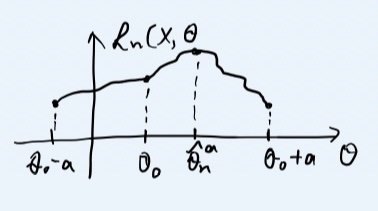
\includegraphics[scale=0.6]{lec2image1}
		\end{center}
		\item $\forall n$ при $w \in S_n$ может существовать целое множество корней $\{\theta_n^{*}\}$. Выберем в этом множестве корень $\hat{\theta_n}$, ближайший к $\theta_0$ (инфимум в множестве корней). Это можно сделать, т.к. функция $\frac{\partial}{\partial \theta} Ln (x, \theta)$ непрерывна по $\theta$, и последовательность корней есть тоже корень. Этот корень $\hat{\theta_n}$ и есть состоятельная оценка $\theta$, покажем это.\\
		$\text{Т.к. } S_n^{\varepsilon} \subseteq S_n, \; (w: |\hat{\theta_n}^{\varepsilon} - \theta_0| < \varepsilon) \subseteq (w: |\hat{\theta_n} - \theta_0| < \varepsilon)$, то для любого малого $\varepsilon > 0$:
		$$P_{\theta_0} (|\hat{\theta_n} - \theta_0| < \varepsilon, S_n) \ge P_{\theta_0}(|\hat{\theta_n}^{\varepsilon} - \theta_0| < \varepsilon, S_n^{\varepsilon})\eqno(3)$$
		$$\begin{gathered}
			\text{Но } P_{\theta_0}(|\hat{\theta_n}^{\varepsilon} - \theta_0| < \varepsilon, S_n^{\varepsilon}) = P_{\theta_0} (S_n^{\varepsilon}) \to 1 \; \Rightarrow \\
			\Rightarrow \text{ в силу } (3) \;  P_{\theta_0} (|\hat{\theta_n} - \theta_0| < \varepsilon, S_n) \to 1 \; \Rightarrow \; \text{пункт } (2) \text{ доказан}. 
		\end{gathered}$$
	\end{enumerate}
\end{Proof}

\begin{remark}\label{lec:2/remark:1}
	Определим следующую величину:
	$$\theta_n^{*} = \begin{cases}
		\text{сост. корень } \hat{\theta_n} \text{ ур-ния правдоподобия, если он} \exists \\
		\theta', \; \theta' \in \Theta, \text{ в противном случае}.
	\end{cases}\eqno(4)$$

	Тогда случайная величина $\theta_n^{*}$ всегда определена и $\theta_n^{*} \xrightarrow[]{P}\theta_0$, т.к. 
	$$P(|\theta_n^{*} - \theta_0| < \varepsilon) = P(|\hat{\theta_n} - \theta_0| < \varepsilon, S_n) + P(|\theta' - \theta| < \varepsilon, \overline{S_n}) \to 1.$$
	Ясно, что $\frac{\partial}{\partial \theta} Ln (x, \theta_n^{*}) = o (1)$, т.к. производная отлична от нуля только на $\overline{S_n}$.
\end{remark}

\begin{definition}\label{lec:2/def:6}
	Будем называть $\theta_n^{*}$ \red{обощенным корнем уравнения правдоподобия} $(2)$.
\end{definition}

\begin{theorem}[\blue{об асимптотической эффективности состоятельного решения}]\label{lec:2/the:3}
	Пусть $X = (X_1, \dots, X_n), \; \{X_i\}$ - н.о.р.с.в. Удовлетворяются условия теоремы Бахадура, в которых условия $(iii)$ и $(vi)$ заменены на предположение о третьей, а не второй производной, т.е. $|\frac{\partial^3}{\partial \theta^3} \ln f(x, \theta)| < M(x) \; \forall x \in N_f, \theta \in \Theta$ и $E_{\theta_0} M(x_1) < \infty$. Тогда, если $\theta_n^{*}$ - обощенный состоятельный корень уравнения правдоподобия из $(4)$, то $\sqrt{n}(\theta_n^{*} - \theta_0) \xrightarrow[]{d}N(0, \frac{1}{i(\theta)})$, т.е. $\theta_n^{*}$ - асимптотически эффективная оценка.
\end{theorem}
\begin{Proof}
	Будем обозначать $\frac{\partial}{\partial \theta}Ln (x, \theta), \frac{\partial^2}{\partial \theta^2}Ln (x, \theta), \dots$ через $Ln' (\theta), Ln^{(2)} (\theta), \dots$.

	Для фиксированного $X$ в силу формулы Тейлора и замечания из предыдущей лекции:
	$$\begin{gathered}
		\overline{o_p}(1) = Ln' (\theta_n^{*}) = Ln' (\theta_0) + Ln^{(2)}(\theta_0) (\theta_n^{*} - \theta_0) + \frac{1}{2} Ln^{(3)} (\tilde{\theta_n}) (\theta_n^{*} - \theta_0)^2, \; \tilde{\theta_n} \in (\theta_0, \theta_n^{*})
	\end{gathered}$$
	После преобразований получаем выражение:
	$$\sqrt{n}(\theta_n^{*} - \theta_0) = -\frac{n^{-\frac{1}{2}}Ln'(\theta_0) + \overline{o_p}(1)}{n^{-1}Ln^{(2)}(\theta_0)+ \frac{1}{2n} Ln^{(3)}(\tilde{\theta_n}) (\theta_n^{*} - \theta_0)}\eqno(5)$$
	Рассмотрим числитель $(5)$:
	$$n^{-\frac{1}{2}}Ln'(\theta_0) = n^{-\frac{1}{2}}\underset{i=1}{\overset{n}{\sum}}\frac{f'_{\theta}(x_i, \theta_0)}{f(x_i, \theta_0)} \xrightarrow[]{d}\xi \sim N(0, i(\theta_0))\eqno(6)$$
	Действительно:
	$$\begin{gathered}
		E_{\theta_0} \frac{f'_{\theta}(x_1, \theta_0)}{f(x_1, \theta_0)} = \underset{N_f}{\overset{}{\int}}\frac{f'_{\theta}(x, \theta_0)}{f(x, \theta_0)}f(x, \theta_0) \nu(dx) = 0\\
		\text{где } N_f \text{носитель плотности вероятности } f, \; f \ge 0\\
		D_{\theta_0}\frac{f'_{\theta}(x_1, \theta_0)}{f(x_1, \theta_0)} = E_{\theta_0} (\frac{\partial}{\partial \theta} \ln f(x_1, \theta_0))^2 = i(\theta_0)
	\end{gathered}$$
	Получаем, что величины $\{\frac{f'_{\theta}(x_i, \theta_0)}{f(x_i, \theta_0)}, i = \ton n\}$ - н.о.р. и соотношение $(6)$ следует из ЦПТ. Т.о. в силу леммы Слуцкого числитель $(5)$ сходится по вероятности к $N(0, i(\theta_0))$.\\

	Рассмотрим знаменатель $(5)$:
	$$n^{-1} Ln^{(2)} (\theta_0) = n^{-1} \underset{i=1}{\overset{n}{\sum}}\left[ \frac{f_{\theta}^{(2)}(x_i, \theta_0)}{f(x_i, \theta_0)}-(\frac{f'_{\theta}(x_i, \theta_0)}{f(x_i, \theta_0)})^2 \right] \xrightarrow[]{P} -i(\theta_0) \eqno(7)$$
	$$\frac{f_{\theta}^{(2)}(x_i, \theta_0)}{f(x_i, \theta_0)}-(\frac{f'_{\theta}(x_i, \theta_0)}{f(x_i, \theta_0)})^2 \text{ - производная от 1-ой производной по правилу Лейбница}$$
	Действительно, в силу ЗБЧ - хотелось бы применить слабый ЗБЧ в форме Чебышева, но там нужна дисперсия, поэтому воспользуемся ЗБЧ в форме Колмогорова, из которого получим сходимость почти наверно:
	$$\begin{gathered}
		\frac{1}{n}\underset{i=1}{\overset{n}{\sum}}\frac{f_{\theta}^{(2) (x, \theta_0)}}{f(x_i, \theta_0)} \xrightarrow[\text{если } \exists \text{ МО}]{P} E_{\theta_0} \frac{f_{\theta}^{(2)} (x_1, \theta_0)}{f(x_1, \theta_0)} = \underset{N_f}{\overset{}{\int}}\frac{f_{\theta}^{(2)} (x, \theta_0)}{f(x, \theta_0)} f(x, \theta_0) \nu(dx) = 0 \\
		\left(\frac{f_{\theta}^{(2) (x, \theta_0)}}{f(x_i, \theta_0)} \text{ - борелевские функции, н.о.р.с.в.}\right)\\
		\frac{1}{n}\underset{i=1}{\overset{n}{\sum}}(\frac{f'_{\theta} (x_i, \theta_0)}{f(x_i, \theta_0)})^2 \xrightarrow[]{P} E_{\theta_0} (\frac{\partial}{\partial \theta}\ln f(x_1, \theta_0))^2 = i(\theta_0)
	\end{gathered}$$
	Применяя лемму Слуцкого, получаем $(7)$ (сходимость к $-i(\theta_0)$).\\

	Рассмотрим второе слагаемое в знаменателе $(5)$:
	$$\begin{gathered}
		\left| \frac{1}{2n} Ln^{(3)} (\tilde{\theta_n}) (\theta_n^{*} - \theta_0) \right| \le \frac{1}{n} |\theta_n^{*} - \theta_0|\cdot \frac{1}{n}\underset{i=1}{\overset{n}{\sum}}M(x_i)\\
		\left(Ln^{(3)} (\tilde{\theta_n}) \le \underset{i=1}{\overset{n}{\sum}}M(x_i) \text{ (из условия)}\right)\\
		|\theta_n^{*} - \theta_0| \xrightarrow[]{P} 0, \; \frac{1}{n}\underset{i=1}{\overset{n}{\sum}}M(x_i) \xrightarrow[]{P} M \text{ - число} \text{ (в силу ЗБЧ)}
	\end{gathered}$$
	Тогда в силу леммы Слуцкого:
	$$\left| \frac{1}{2n} Ln^{(3)} (\tilde{\theta_n}) (\theta_n^{*} - \theta_0) \right| \xrightarrow[]{P}0\eqno(8)$$
	В силу $(7)$ и $(8)$ и леммы Слуцкого знаменатель в $(5)$ сходится по вероятности к $-i(\theta_0)$.\\
	Значит, по лемме Слуцкого вся дробь $(5)$ сходится по распределению к 
	$\frac{1}{i(\theta_0)} \xi \sim N(0, \frac{i(\theta_0)}{i^2 (\theta_0)}) = N(0, \frac{1}{i(\theta_0)})$, где $\xi$ - гауссовская случайная величина.
\end{Proof}

\section{ОМП для векторного параметра}\label{lec:3/sec:2}

Пусть $X = (X_1, \dots, X_n)$ - н.о.р., $X_1 \sim f(x, \theta)$, $\theta \in \Theta \subseteq \mathbb{R}^k$, $\Theta$ - открытое множество.\\

Логарифмическое правдоподобие имеет вид:
$$Ln (x, \theta) = \underset{i=1}{\overset{n}{\sum}}\ln f(x_i, \theta)$$
Система уравнений правдоподобия имеет вид:
$$\frac{\partial Ln (x, \theta)}{\partial \theta_i}=0, \; i=\ton k\eqno(9)$$
При условиях регулярности, похожих на условия теоремы \ref{lec:3/sec:1}, показывается:
\begin{enumerate}
	\item с вероятностью, стремящейся к $1$ при $n \to \infty$, система уравнений $(9)$ имеет такое решение $\hat{\theta_n} \in \Theta$, что $\hat{\theta_n}$ сходится к истинному значению $\theta_0$
	\item соответствующая оценка $\theta_n^{*}$ асимптотически нормальна, а именно:
	$$\begin{gathered}
		\sqrt{n} (\theta_n^{*} - \theta_0) \xrightarrow[n \to \infty]{d}N(o, I^{-1}(\theta_0))\\
		I(\theta) > 0 \text{ - \blue{матрица информации Фишера, }} I(\theta) = (I_{ij} (\theta)) \\
		I_{ij}(\theta) = E_{\theta} \left( \frac{\partial \ln f(x, \theta)}{\partial \theta_i} \cdot \frac{\partial \ln f(x, \theta)}{\partial \theta_j} \right)
	\end{gathered}$$
\end{enumerate}

\section{АЭО для интервала}\label{lec:3/sec:3}

\begin{example}\label{lec:3/example:1}
	Пусть $X = (X_1, \dots, X_n)$, где $\{X_i\}$ - н.о.р., $X_1 \sim N(\theta, \sigma^2), \; a < \theta < b$, т.е. $\Theta = (a,b)$. $a$ и $b$ - известные конечные числа, $\theta$ неизвестно, $\sigma^2$ известно. Необходимо построить АЭО.
\end{example}
\begin{solution}
	Построим АЭО $\theta_n^{*}$ для $\theta$.
	$$\begin{gathered}
		p(x, \theta) = (\frac{1}{\sqrt{2 \pi} \sigma})^n e^{-\frac{1}{2\sigma^2}\underset{i=1}{\overset{n}{\sum}}(x_i - \theta)^2} \text{ - плотность вероятности гауссовской сл. в.}\\
		Ln (x, \theta) = \ln (\frac{1}{\sqrt{2 \pi} \sigma})^n - \frac{1}{2 \sigma^2} \underset{i=1}{\overset{n}{\sum}}(x_i - \theta)^2\\
		- \frac{1}{2 \sigma^2} \underset{i=1}{\overset{n}{\sum}}(x_i - \theta)^2 \text{ - парабола ветвями вниз}
	\end{gathered}$$
	Уравнение правдоподобия имеет вид:
	$$\frac{\partial Ln (x, \theta)}{\partial \theta} = \frac{1}{\sigma^2}\underset{i=1}{\overset{n}{\sum}}(x_i - \theta) = 0$$
	Решение существует и единственно - это $\overline{X}$, причем в точке $\theta = \overline{X}$ функция $Ln (x, \theta)$ достигает максимума, т.к.:
	$$\frac{\partial^2 Ln(x, \overline{X})}{\partial \theta^2} = -\frac{1}{\sigma^2} < 0$$
	Т.о., если $a < \overline{X} < b$, то ОМП существует с вероятностью, стремящейся к $1$ и равна $\overline{X}$, в противном случае ОМП не существует.\\

	Если положить:
	$$\theta_n^{*} = \begin{cases}
		\overline{X}, \; a < \overline{X} < b \\
		\frac{a+b}{2} \text{ (любое число), } \overline{X} \not \in (a, b) 
	\end{cases}\eqno(9)$$
	то в силу теоремы \ref{lec:3/sec:1} (условия выполнены) $\theta_n^{*}$ - АЭО, т.е.:
	$$\sqrt{n}(\theta_n^{*} - \theta_0) \xrightarrow[]{d} N(0, \sigma^2), \; i(\theta) = \frac{1}{\sigma^2}\eqno(10)$$
	(также $(10)$ можно проверить непосредственно)
\end{solution}

\begin{remark}\label{lec:3/remark:1}
	Если $\theta \in [a,b]$, то по тоереме Вейерштрасса непрерывная функция на компакте достигает максимума и минимума. Тогда:
	$$\theta_n^{*} = \begin{cases}
		\overline{X}, \; \overline{X} \in (a, b)\\
		a, \; \overline{X} < a \\
		b, \; \overline{X} > b
	\end{cases}$$
	В $\theta = a$ или $\theta = b$ нет асимптотической гауссовости, поэтому надо рассматривать только открытые множества.
\end{remark}



